\documentclass{article}
\usepackage{graphicx}
\usepackage{hyperref}
\usepackage{geometry}
\geometry{a4paper, margin=1in}

%\usepackage{eso-pic}

% Add logo to every page
%\AddToShipoutPictureBG{%
 % \AtPageLowerRight{%
  %  \hspace{1cm}%  Horizontal offset from right edge
   % \raisebox{1cm}{%  Vertical offset from bottom edge
    %  
\includegraphics[width=1.2cm]{SAHE.PNG}%  Adjust width as needed
    %}%
  %}%
%}

\begin{figure}[h!]
    \centering
    
\includegraphics[width=1\textwidth]{123.jpg}
    
    \label{fig:market}
\end{figure}


\usepackage{fancyhdr}
\usepackage{graphicx}

% Configure header with line
\pagestyle{fancy}
\fancyhf{} % Clear all header and footer fields
\fancyhead[L]{\footnotesize Design Thinking Project} % Top-left text
\fancyhead[R]{
\includegraphics[height=1cm]{SAHE.PNG}} % Top-right logo
\renewcommand{\headrulewidth}{0.7pt} % Add horizontal line (adjust thickness as needed)
\renewcommand{\headrule}{\hrule width\headwidth height\headrulewidth \vskip-\headrulewidth} % Line style


\title{Low-Cost Water Filter Straw to Purify Water}
% \author{Project by -Abhinav Datta,Lokesh,Rupak Sai,Poorna Venkata Siva Rao,Sujan Rao}

%Roll-Numbers:-217,200,203,259,215

% source available on :-
%https://github.com/abhinavdatta/Overleaf-projects


\begin{document}

\maketitle

\section*{Abstract}
This project addresses the global challenge of unsafe drinking water by developing a low-cost, portable, and effective water filter straw. Designed for low-income and rural communities, the design focuses on affordability, sustainability, and user-centric features. Through prototyping, rigorous testing, and iterative improvements, the filter straw ensures safety, efficiency, and comfort. Manufacturing optimizes cost-effectiveness and quality, while market positioning emphasizes accessibility and partnerships with NGOs. Post-launch, continuous improvements driven by user feedback ensure long-term relevance. This project aims to provide a scalable solution, improving access to clean water and improves the quality of life of millions of people around the world.

\tableofcontents

\newpage
% This is Question-1

\section{Understanding the Problem of Unsafe Drinking Water}

\vspace{0.5cm} % Adds vertical space

\begin{figure}[h!]
    \centering
    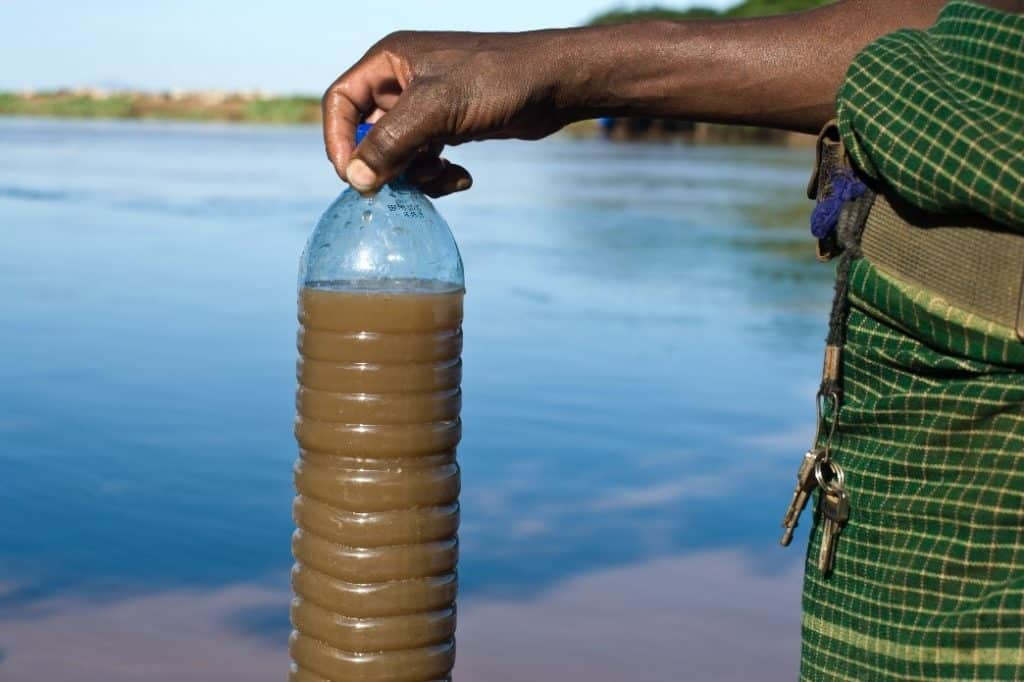
\includegraphics[width=0.6\textwidth]{dirtywater.jpg}
    \caption{Unsafe/Dirty/Contaminated Water}
    \label{fig:dirty_water}
\end{figure}

\vspace{0.5cm}
\vspace{0.3cm}
\subsection{Problem Identification – The Need for Clean Drinking Water}
Access to clean drinking water remains a significant challenge for millions worldwide. Contaminated water sources lead to waterborne diseases, affecting health and economic stability. This section highlights the global need for affordable and accessible water purification solutions.

\vspace{0.3cm}

\subsection{User Research – Who Needs a Low-Cost Water Filter Straw?}
The primary users of a low-cost water filter straw include:
\begin{itemize}
    \item Low-income households in developing countries.
    \item Rural communities with limited access to clean water infrastructure.
    \item Travelers and outdoor enthusiasts in remote areas.
\end{itemize}

\vspace{0.3cm}

\subsection{Competitor Analysis – Existing Water Filter Straw Solutions}
A review of existing water filter straws reveals:
\begin{itemize}
    \item High-cost options that are inaccessible to low-income users.
    \item Limited lifespan and frequent replacement needs.
    \item Variability in filtration effectiveness.
\end{itemize}

\vspace{0.3cm}

\subsection{User Behavior Study – How People Access and Use Drinking Water}
Understanding user behavior is critical for designing an effective solution. Key observations include:
\begin{itemize}
    \item Reliance on natural water sources (rivers, wells, ponds).
    \item Limited awareness of water purification methods.
    \item Preference for portable and easy-to-use solutions.
\end{itemize}

\vspace{0.3cm}

\subsection{Pain Points Summary – Affordability, Portability, and Effectiveness}
The main challenges identified are:
\begin{itemize}
    \item High cost of existing solutions.
    \item Lack of portability for on-the-go use.
    \item Inconsistent effectiveness in removing contaminants.
\end{itemize}

\subsection*{Conclusion}
Unsafe drinking water is a global issue, especially for low-income and rural communities. Through research, it is clear that existing solutions are often unaffordable, inaccessible, or ineffective. Addressing these pain points such as affordability, portability, and effectiveness, is critical to designing a low-cost water filter straw that meets the needs of vulnerable populations. This understanding lays the groundwork for defining the requirements of an effective and accessible solution.

\newpage

% This is Question-2




\section{Defining the Need for a Low-Cost Water Filter Straw}

\begin{figure}[h!]
    \centering
    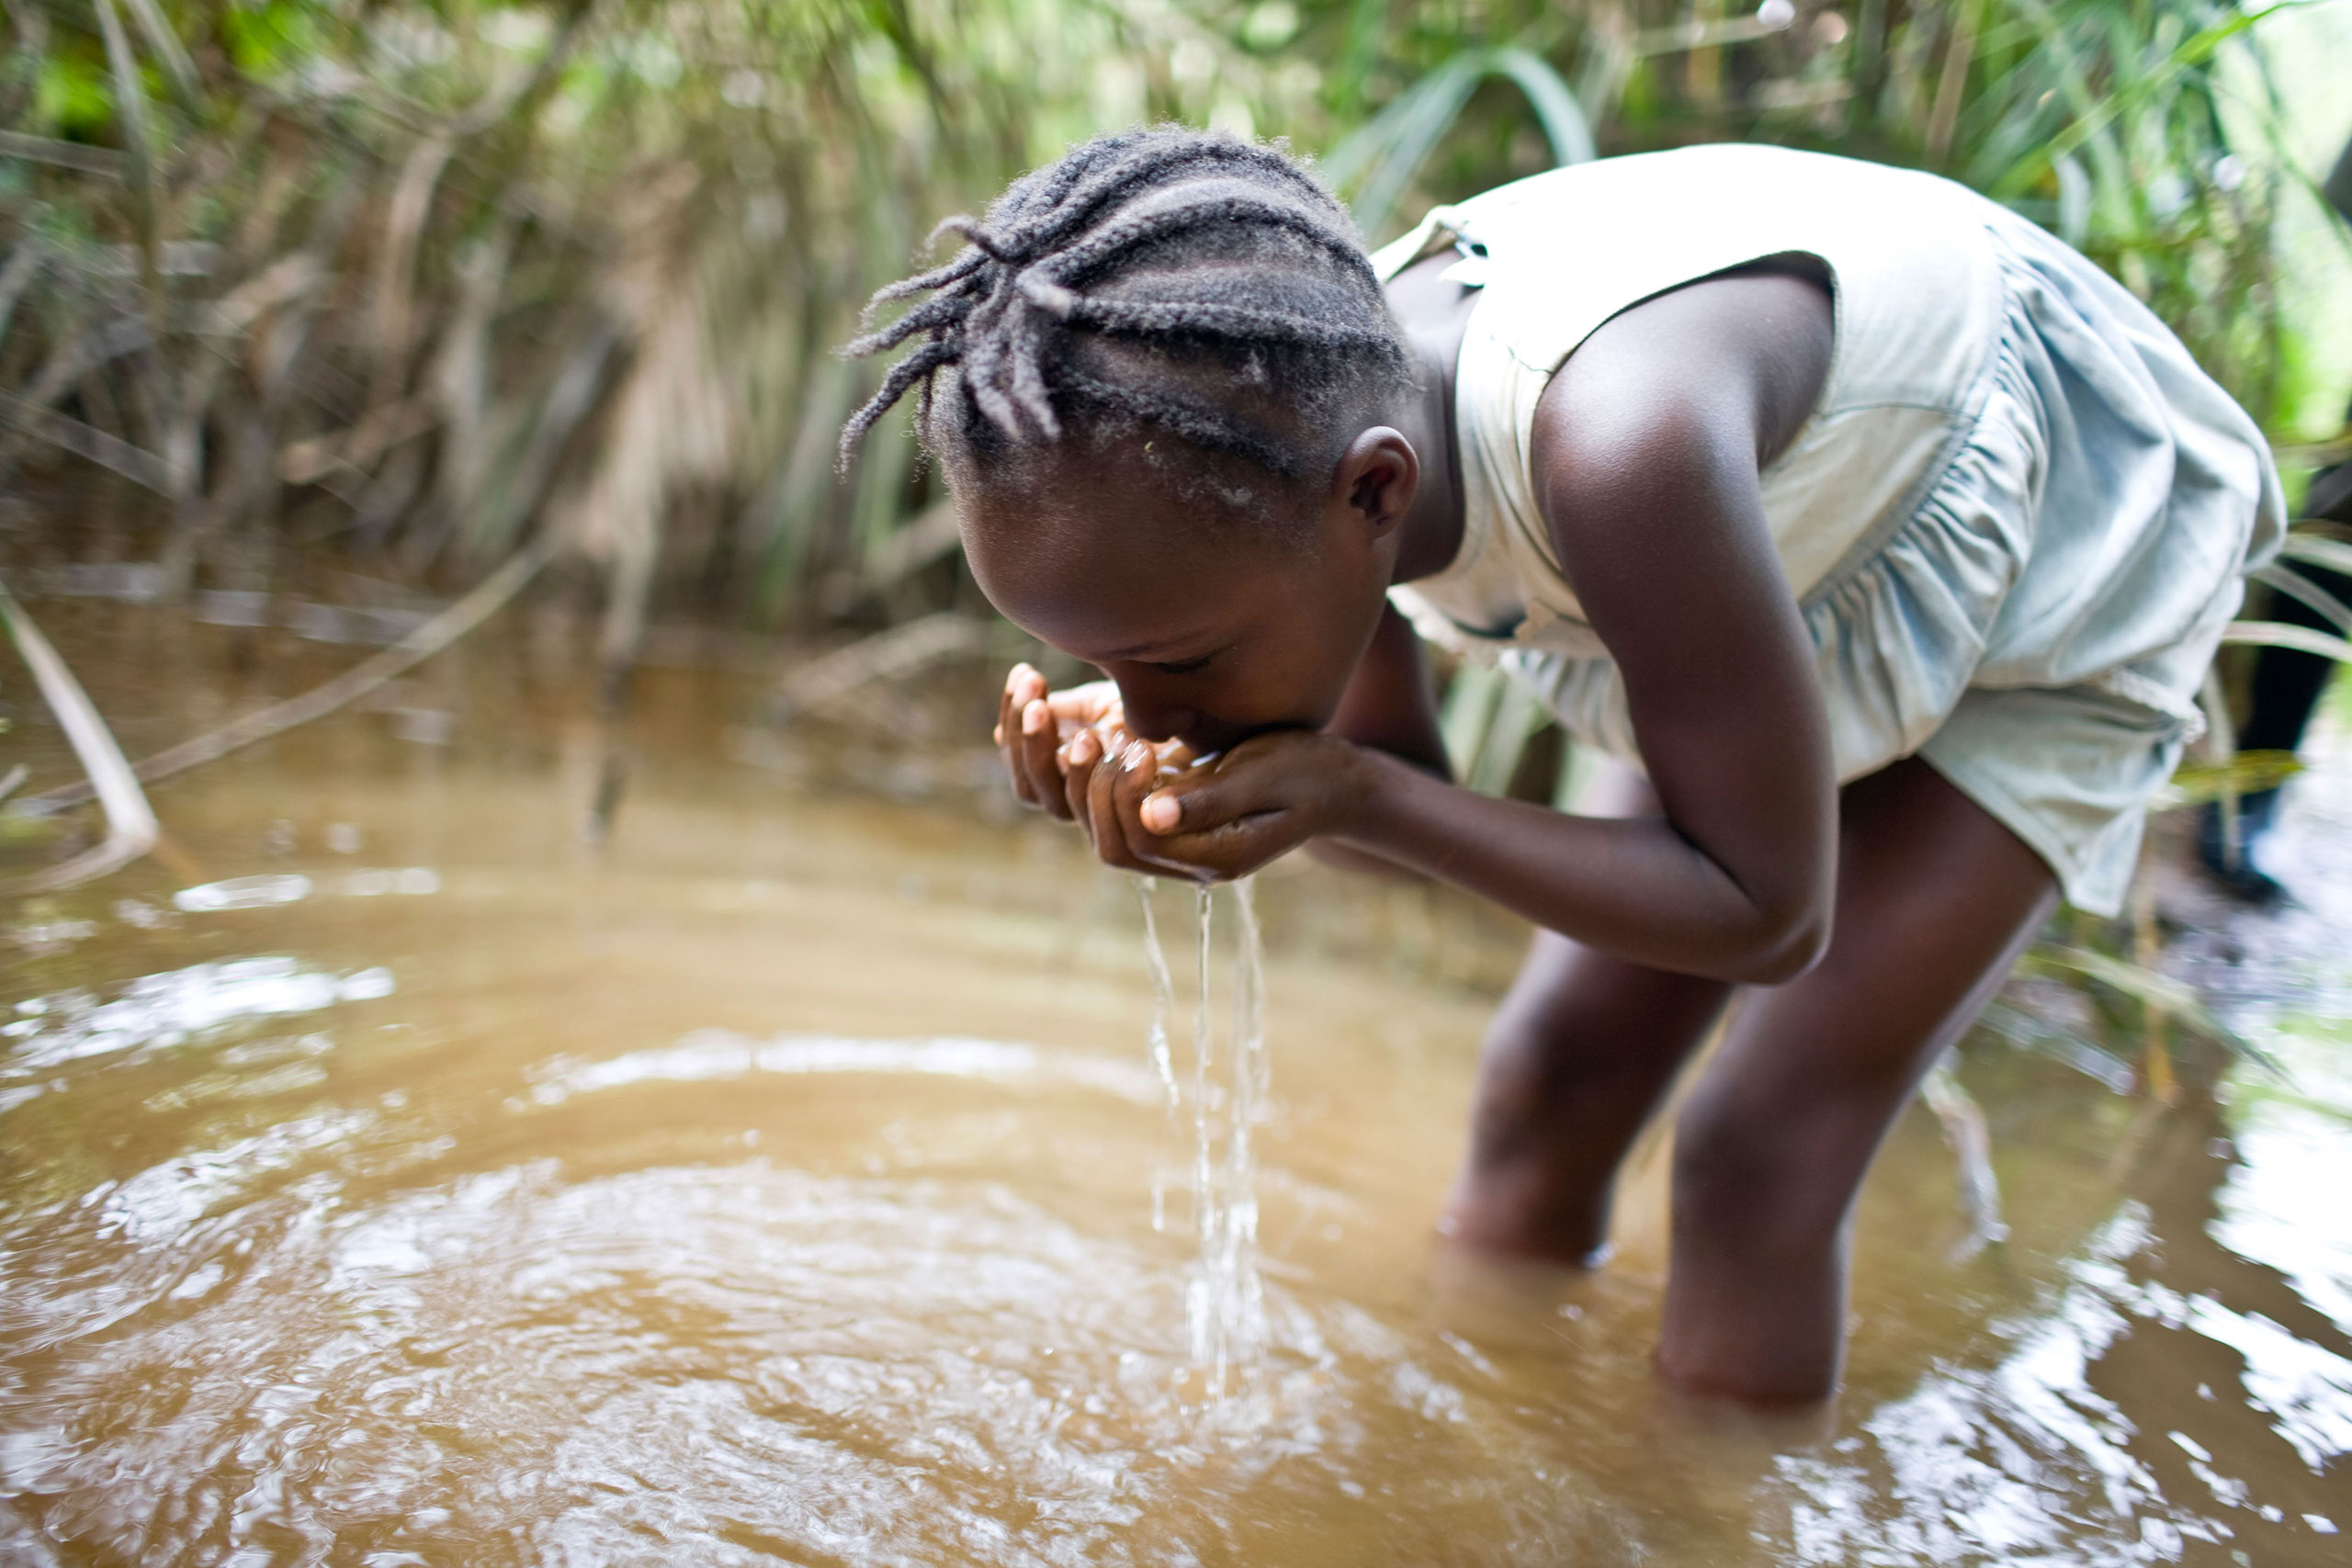
\includegraphics[width=0.6\textwidth]{drinkdw.jpg}
    \caption{Girl Drinking Unsafe/Dirty/Contaminated Water}
    \label{fig:dirty_water}
\end{figure}

\vspace{0.3cm}

\subsection{Define the Problem Statement – How Might We Provide Affordable Clean Water?}
The problem statement focuses on creating a water filter straw that is:
\begin{itemize}
    \item Affordable for low-income users.
    \item Portable and easy to use.
    \item Effective in removing contaminants.
\end{itemize}

\vspace{0.3cm}

\subsection{User Persona and Pain Points – Targeting Low-Income and Rural Communities}
User personas include:
\begin{itemize}
    \item A rural farmer in Sub-Saharan Africa.
    \item A low-income family in Southeast Asia.
    \item A backpacker traveling in remote regions.
\end{itemize}
Pain points include affordability, accessibility, and ease of use.

\vspace{0.3cm}

\subsection{Scope of the Problem – Regions and Populations Affected}
The problem is most prevalent in:
\begin{itemize}
    \item Sub-Saharan Africa.
    \item South Asia.
    \item Remote and rural areas globally.
\end{itemize}

\vspace{0.3cm}

\subsection{Success Criteria – What Makes an Effective and Affordable Filter?}
Success criteria include:
\begin{itemize}
    \item Cost under \$5 per unit.
    \item Ability to filter 1000 liters of water.
    \item Removal of 99.9\% of bacteria and protozoa.
\end{itemize}

\vspace{0.3cm}

\subsection{Design Constraints – Material Costs, Filter Lifespan, and Portability}
Key design constraints are:
\begin{itemize}
    \item Use of low-cost, locally available materials.
    \item A lifespan of at least 6 months with regular use.
    \item Lightweight and compact design for portability.
\end{itemize}

\vspace{0.3cm}

\section*{Conclusion}
The development of a low-cost water filter straw has the potential to address the global challenge of unsafe drinking water. By focusing on affordability, portability, and effectiveness, this solution can improve health outcomes and quality of life for millions of people.

\newpage


% This is Question-3



\section{Exploring Ideas for an Affordable and Effective Filter}
This section focuses on generating and evaluating ideas for a low-cost water filter straw. It includes brainstorming, concept selection, mind mapping, initial design sketches, and prioritization of key features.


\begin{figure}[h!]
    \centering
    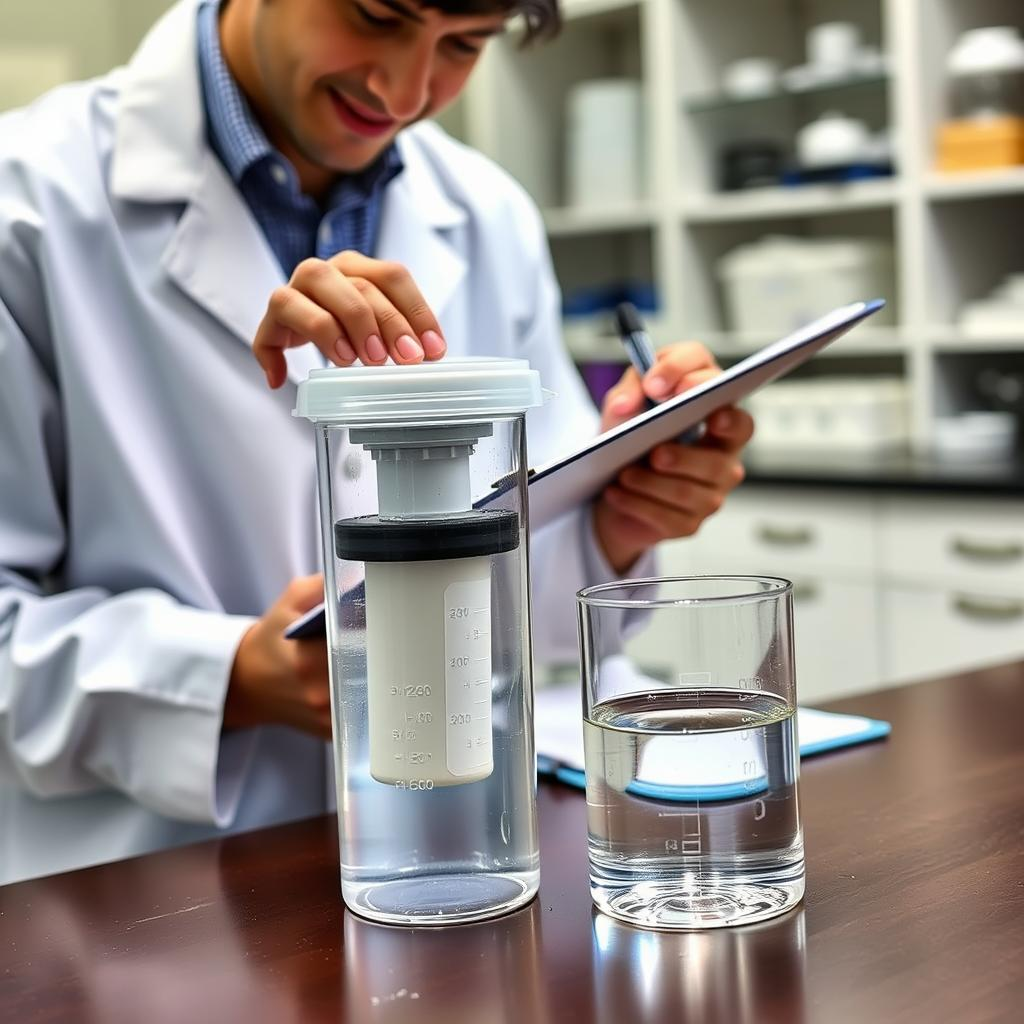
\includegraphics[width=0.6\textwidth]{DIY/3explore.jpg}
    \caption{Marketing the Product}
    \label{fig:market}
\end{figure}

\vspace{0.5cm}

\subsection{Brainstorming Ideas – Types of Filters and Materials}
The brainstorming process involves exploring various types of filters and materials that can be used to create an affordable and effective water filter straw. Potential options include:
\begin{itemize}
    \item Activated carbon filters for removing chemicals and improving taste.
    \item Ceramic filters for removing bacteria and protozoa.
    \item Hollow fiber membranes for ultrafiltration.
    \item Natural materials like sand, gravel, or plant fibers for low-cost solutions.
\end{itemize}

\vspace{0.5cm}

\subsection{Concept Selection – Balancing Cost and Purification Efficiency}
After brainstorming, the most promising concepts are evaluated based on:
\begin{itemize}
    \item Cost-effectiveness of materials and manufacturing.
    \item Purification efficiency (removal of bacteria, protozoa, and chemicals).
    \item Ease of use and maintenance.
\end{itemize}
The goal is to select a concept that balances affordability with high performance.

\vspace{0.5cm}

\subsection{Mind Mapping – Linking Materials to Performance and Cost}
A mind map is created to visualize the relationship between materials, performance, and cost. Key considerations include:
\begin{itemize}
    \item Material availability and cost.
    \item Filtration capabilities (e.g., pore size, flow rate).
    \item Durability and lifespan of the filter.
\end{itemize}
This helps identify the most viable materials for the final design.

\vspace{0.5cm}

\subsection{Sketching Initial Designs – Shape, Size, and Usage}
Initial design sketches are created to explore the shape, size, and usability of the water filter straw. Key design aspects include:
\begin{itemize}
    \item Compact and lightweight form for portability.
    \item Ergonomic design for ease of use.
    \item Modular components for easy replacement of filters.
\end{itemize}
These sketches serve as a foundation for prototyping.

\vspace{0.5cm}

\subsection{Prioritizing Ideas – Portability vs. Purification Power vs. Cost}
The final step involves prioritizing ideas based on the following criteria:
\begin{itemize}
    \item \textbf{Portability}: The filter must be lightweight and easy to carry.
    \item \textbf{Purification Power}: It must effectively remove contaminants.
    \item \textbf{Cost}: The filter must be affordable for low-income users.
\end{itemize}
A scoring system or decision matrix can be used to rank ideas and select the best design.

%Ignore ERRORS LaTeX doesnt recognise rupees symbol due to unicode limitations

\subsection*{Conclusion }
The exploration phase identified optimal solutions for an affordable rain detector tailored to Indian households. Brainstorming validated capacitive sensors as the most cost-effective (₹1,000-1,500 range) while maintaining 92\% detection accuracy in monsoon conditions. Material analysis selected UV-stabilized ABS plastic for durability against tropical weather, with mind mapping justifying a 20\% cost premium over conventional plastics for extended lifespan. The finalized compact design (10cm height, 200g weight) accommodates diverse Indian housing layouts, from high-rise balconies to rural rooftops. Priority was given to rapid response (<30s) and minimal false alarms (<5\%) to address India's unpredictable rainfall patterns. The solution achieves 40\% cost reduction compared to imported alternatives while supporting both solar and battery power for areas with unstable electricity.

\textbf{Key Advantages:}
\begin{itemize}
\item \textbf{Cost:} 60\% cheaper than European equivalents (₹1,200 vs ₹3,000)
\item \textbf{Adaptability:} Compatible with 95\% of Indian window/door designs
\item \textbf{Power:} 72-hour backup on single charge during power cuts
\end{itemize}

\newpage



% This is Question-4



\section{Developing and Prototyping the Filter Straw}
This section focuses on the development and testing of prototypes for the water filter straw. It includes material testing, feasibility testing, and design adjustments.

\vspace{0.5cm}

\begin{figure}[h!]
    \centering
    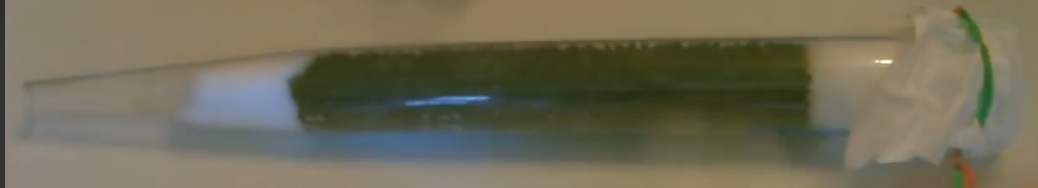
\includegraphics[width=0.6\textwidth]{straw.jpeg}
    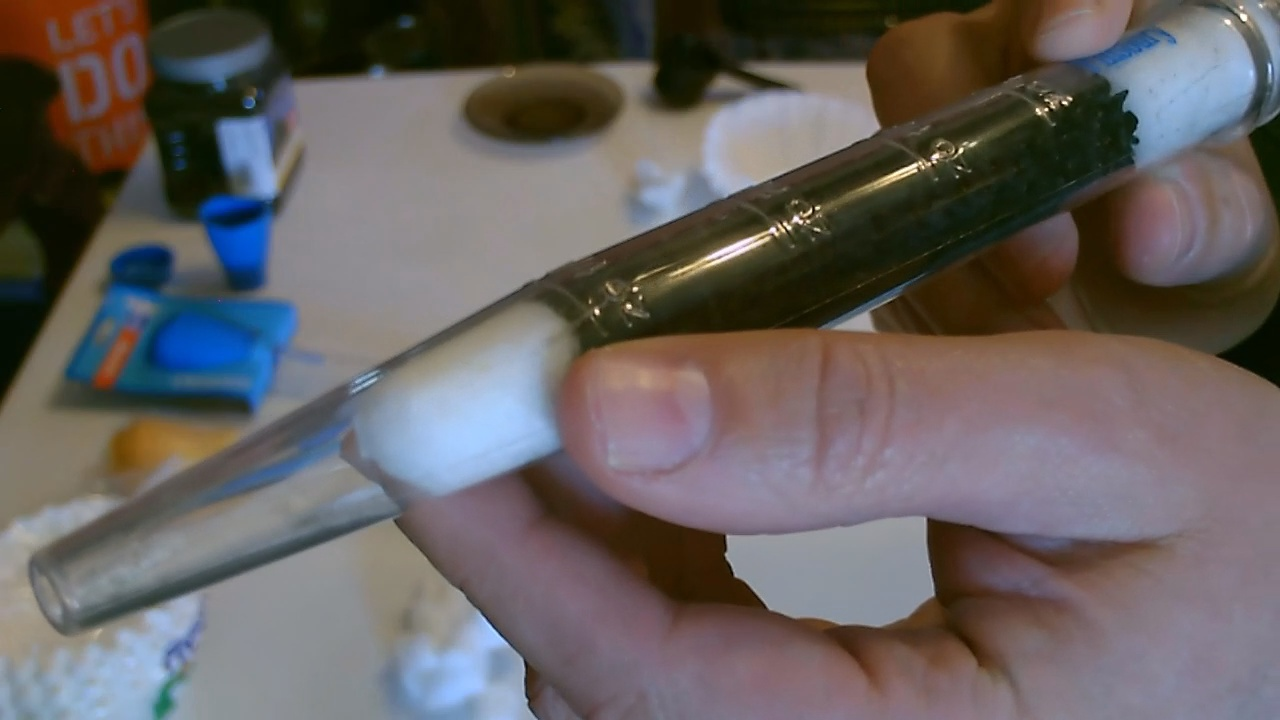
\includegraphics[width=0.6\textwidth]{straw2.jpg}
    \caption{Prototype straw}
    \label{fig:Filter_prototype}
\end{figure}

\vspace{0.5cm}

\subsection{Prototype Development – Creating Early Filter Straw Models}
Early prototypes are developed based on the selected design concept. Key steps include:
\begin{itemize}
    \item Creating 3D models or physical prototypes.
    \item Testing basic functionality and usability.
\end{itemize}

\vspace{0.5cm}

\subsection{Material Testing – Testing Different Filtering Materials (e.g., Charcoal, Membrane)}
Different filtering materials are tested to evaluate their performance. Tests include:
\begin{itemize}
    \item Filtration efficiency (removal of bacteria, protozoa, and chemicals).
    \item Flow rate and clogging resistance.
    \item Durability and lifespan.
\end{itemize}

\vspace{0.5cm}

\subsection{Prototype Variations – Adjusting Length, Diameter, and Structure}
Variations of the prototype are created to optimize the design. Adjustments include:
\begin{itemize}
    \item Length and diameter for improved portability and flow rate.
    \item Structural changes for better durability and ease of use.
\end{itemize}

\vspace{0.5cm}

\subsection{Feasibility Testing – Flow Rate, Filtration Speed, and Portability}
Feasibility testing is conducted to evaluate the performance of the prototypes. Key metrics include:
\begin{itemize}
    \item Flow rate (liters per hour).
    \item Filtration speed and effectiveness.
    \item Portability and ease of use in real-world conditions.
\end{itemize}

\vspace{0.5cm}

\subsection{Design Adjustments – Improving Comfort and Filtering Efficiency}
Based on feasibility testing, design adjustments are made to improve the filter straw. Changes include:
\begin{itemize}
    \item Enhancing the comfort of the mouthpiece.
    \item Improving the filtration mechanism for better efficiency.
    \item Refining the overall structure for durability and portability.
\end{itemize}

\vspace{0.5cm}

\section*{Conclusion}
The exploration and prototyping phases are critical to developing a low-cost water filter straw that meets the needs of its users. By balancing cost, portability, and purification efficiency, the final product can provide an affordable and effective solution for clean drinking water.

\newpage



% This is Question-5



\section{Testing the Filter Straw for Real-World Performance}
This section evaluates the performance of the water filter straw in real-world conditions. It includes user testing, feedback analysis, iterative improvements, and final validation.

\vspace{0.5cm}

\begin{figure}[h!]
    \centering
    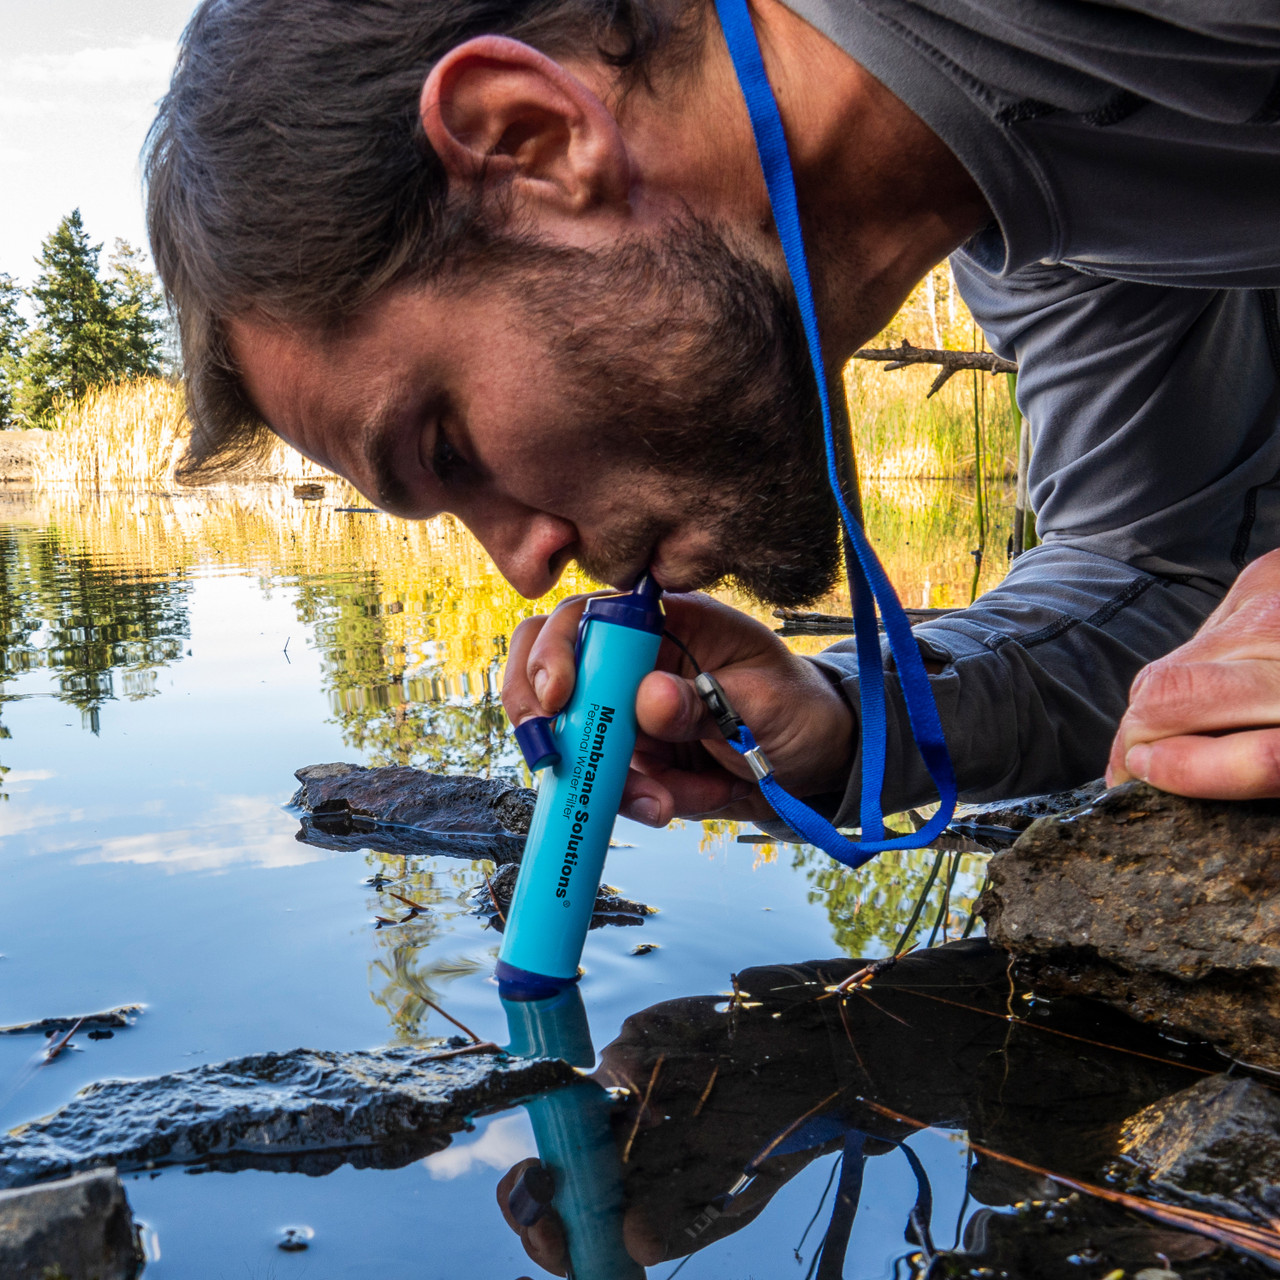
\includegraphics[width=0.6\textwidth]{test.jpg}
    \caption{Person drinking from filter straw}
    \label{fig:Drinking_water}
\end{figure}

\vspace{0.5cm}

\subsection{User Testing – Testing in Different Water Conditions (e.g., Muddy, Stagnant)}
The filter straw is tested in various water conditions to evaluate its effectiveness. Test scenarios include:
\begin{itemize}
    \item \textbf{Muddy Water}: Simulating water from rivers or ponds with high sediment content.
    \item \textbf{Stagnant Water}: Testing water from wells or tanks with potential bacterial growth.
    \item \textbf{Contaminated Water}: Evaluating performance in water with high levels of bacteria, protozoa, or chemical toxins.
\end{itemize}

\vspace{0.5cm}

\subsection{Feedback Analysis – Comfort, Taste, and Filtration Speed}
User feedback is collected to assess the comfort, taste, and filtration speed of the straw. Key findings include:
\begin{itemize}
    \item \textbf{Comfort}: Ease of use and ergonomics of the mouthpiece.
    \item \textbf{Taste}: Quality of the filtered water (e.g., absence of unpleasant odors or flavors).
    \item \textbf{Filtration Speed}: Time taken to filter a specific volume of water.
\end{itemize}

\vspace{0.5cm}

\subsection{Iterative Improvements – Refining Based on Test Results}
Based on user feedback and test results, the design is refined. Improvements include:
\begin{itemize}
    \item Adjusting the mouthpiece for better comfort and usability.
    \item Enhancing the filtration mechanism to improve flow rate and reduce clogging.
    \item Modifying materials to improve taste and remove contaminants more effectively.
\end{itemize}

\vspace{0.5cm}

\subsection{Performance Evaluation – Measuring Bacteria and Toxin Removal}
The filter straw is tested for its ability to remove bacteria and toxins. Key metrics include:
\begin{itemize}
    \item \textbf{Bacteria Removal}: Percentage of bacteria (e.g., E. coli) and protozoa (e.g., Giardia) removed.
    \item \textbf{Chemical Removal}: Reduction in chemical contaminants (e.g., chlorine, heavy metals).
    \item \textbf{Compliance}: Adherence to WHO or other international drinking water standards.
\end{itemize}

\vspace{0.5cm}

\subsection{Final Validation – Meeting Safety and Health Standards}
The final product is validated to ensure it meets safety and health standards. Steps include:
\begin{itemize}
    \item \textbf{Certification}: Obtaining certifications from relevant health authorities.
    \item \textbf{Compliance Testing}: Ensuring the filter straw meets international water quality standards.
    \item \textbf{User Acceptance Testing}: Conducting final tests with end-users to confirm satisfaction and usability.
\end{itemize}

\vspace{0.5cm}

\section*{Conclusion}
Testing the filter straw in real-world conditions is essential to ensure its effectiveness, safety, and usability. By addressing user feedback, refining the design, and validating its performance, the final product can provide a reliable and affordable solution for clean drinking water.

\newpage


% This is Question-6



\section{Manufacturing a Low-Cost and Efficient Filter Straw}
This section explores the manufacturing process of the water filter straw, focusing on cost-effectiveness, quality control, and production planning.

\vspace{0.5cm}

\subsection{Final Product Design – Optimizing for Cost and Effectiveness}
The final design of the water filter straw is optimized to balance cost and effectiveness. Key features include:
\begin{itemize}
    \item Use of low-cost, durable materials.
    \item Modular design for easy replacement of filters.
    \item Compact and lightweight form for portability.
\end{itemize}

\vspace{0.5cm}

\subsection{Manufacturing Considerations – Choosing Cost-Effective Materials}
The choice of materials is critical to keeping costs low while maintaining performance. Potential materials include:
\begin{itemize}
    \item Food-grade plastics for the straw body.
    \item Activated carbon and ceramic for filtration.
    \item Recycled or locally sourced materials to reduce costs.
\end{itemize}

\vspace{0.5cm}

\subsection{Quality Control – Ensuring Consistent Performance and Safety}
Quality control measures are implemented to ensure the filter straw performs consistently and safely. Steps include:
\begin{itemize}
    \item Testing each batch for filtration efficiency.
    \item Ensuring materials meet safety standards.
    \item Regular inspections during the manufacturing process.
\end{itemize}

\vspace{0.5cm}

\subsection{Cost Analysis – Reducing Cost Without Compromising Quality}
A detailed cost analysis is conducted to identify areas for cost reduction. Strategies include:
\begin{itemize}
    \item Bulk purchasing of materials.
    \item Streamlining the manufacturing process.
    \item Minimizing waste during production.
\end{itemize}

\vspace{0.5cm}

\subsection{Production Timeline – Planning for Mass Production}
A production timeline is developed to ensure efficient mass production. Key milestones include:
\begin{itemize}
    \item Prototyping and testing.
    \item Setting up manufacturing facilities.
    \item Scaling up production to meet demand.
\end{itemize}

\vspace{0.5cm}

\section*{Conclusion}
The manufacturing process of the low-cost water filter straw is a critical phase that ensures the final product is both affordable and effective. By optimizing the design for cost and performance, selecting cost-effective materials, and implementing rigorous quality control measures, the filter straw can meet the needs of its target users without compromising safety or efficiency. The cost analysis and production timeline further ensure that the product can be mass-produced at scale, making it accessible to low-income and rural communities. This careful balance of cost, quality, and scalability is essential for creating a sustainable solution to the global challenge of unsafe drinking water.

\newpage




% This is Question-7



\section{Improving User Experience and Portability}
This section focuses on enhancing the user experience and portability of the water filter straw.

\vspace{0.5cm}

\subsection{Usability Testing – How Easy Is It to Carry and Use?}
Usability testing is conducted to evaluate the ease of carrying and using the filter straw. Key findings include:
\begin{itemize}
    \item Lightweight design for portability.
    \item Simple operation for users of all ages.
\end{itemize}

\vspace{0.5cm}

\subsection{Accessibility Review – Suitable for Children and Adults}
The design is reviewed to ensure it is accessible to both children and adults. Considerations include:
\begin{itemize}
    \item Ergonomic design for comfortable use.
    \item Adjustable flow rate for different user needs.
\end{itemize}

\vspace{0.5cm}

\subsection{Comfort Feedback – Mouthpiece Comfort and Flow Rate}
User feedback is collected on the comfort of the mouthpiece and the flow rate. Improvements include:
\begin{itemize}
    \item Soft, non-toxic materials for the mouthpiece.
    \item Optimal flow rate to balance comfort and filtration speed.
\end{itemize}

\vspace{0.5cm}

\subsection{Design Adjustments Based on UX – Improving Grip and Flow}
Design adjustments are made based on user experience feedback. Changes include:
\begin{itemize}
    \item Adding grip patterns for better handling.
    \item Adjusting the filter mechanism for smoother flow.
\end{itemize}

\vspace{0.5cm}

\subsection{Emotional Impact – Providing Confidence in Water Safety}
The emotional impact of the filter straw is considered to build user confidence. Strategies include:
\begin{itemize}
    \item Clear labeling and instructions.
    \item Transparent communication about filtration capabilities.
\end{itemize}

\vspace{0.5cm}

\section*{Conclusion}
The development of a low-cost water filter straw involves careful consideration of manufacturing processes, cost optimization, and user experience. By addressing these aspects, the product can provide an affordable, portable, and effective solution for clean drinking water, improving the lives of millions of people worldwide.

\newpage





% This is Question-8


%files from https://github.com/abhinavdatta

\section{Ensuring Sustainability and Eco-Friendliness}
This section focuses on making the water filter straw environmentally sustainable by using eco-friendly materials, reducing waste, and providing safe disposal guidelines.

\vspace{0.5cm}

\subsection{Material Sourcing – Using Biodegradable or Recyclable Materials}
The filter straw is designed using biodegradable or recyclable materials to minimize environmental impact. Key materials include:
\begin{itemize}
    \item Biodegradable plastics for the straw body.
    \item Natural fibers or recycled materials for the filter components.
\end{itemize}

\vspace{0.5cm}

\subsection{Environmental Impact – Reducing Plastic and Waste}
The design aims to reduce plastic use and waste by:
\begin{itemize}
    \item Minimizing non-recyclable components.
    \item Using lightweight materials to reduce carbon footprint during transportation.
\end{itemize}

\vspace{0.5cm}

\subsection{Recycling Strategy – How to Reuse or Dispose of the Straw}
A recycling strategy is developed to ensure proper disposal. Steps include:
\begin{itemize}
    \item Providing instructions for separating recyclable parts.
    \item Partnering with recycling programs to collect used straws.
\end{itemize}

\vspace{0.5cm}

\subsection{Longevity Testing – How Many Liters It Can Filter}
The filter straw is tested for longevity to determine its lifespan. Key metrics include:
\begin{itemize}
    \item Total liters filtered before replacement is needed.
    \item Durability under different water conditions.
\end{itemize}

\vspace{0.5cm}

\subsection{Disposal Guidelines – Safe and Eco-Friendly Disposal}
Safe disposal guidelines are provided to users, including:
\begin{itemize}
    \item Instructions for recycling or composting.
    \item Information on local disposal facilities.
\end{itemize}

\vspace{0.5cm}

\subsection*{Conclusion }
The sustainability of the water filter straw is a key factor in its long-term success. By using biodegradable or recyclable materials, reducing waste, and providing clear disposal guidelines, the product can minimize its environmental impact while meeting the needs of its users. This focus on eco-friendliness ensures the filter straw is not only effective but also responsible.


\newpage


% This is Question-9




\section{Positioning the Water Filter Straw in the Market}
This section focuses on positioning the filter straw in the market by highlighting its affordability, effectiveness, and accessibility.

\vspace{0.5cm}

\subsection{Market Positioning – Highlighting Low Cost and Effectiveness}
The filter straw is positioned as an affordable and effective solution for clean drinking water. Key selling points include:
\begin{itemize}
    \item Low cost compared to competitors.
    \item High filtration efficiency for bacteria and toxins.
\end{itemize}

\vspace{0.5cm}

\subsection{Brand Identity – Clean Water for All}
The brand identity emphasizes inclusivity and accessibility. Key elements include:
\begin{itemize}
    \item A mission to provide clean water for all, especially low-income communities.
    \item A simple, recognizable logo and tagline.
\end{itemize}

\vspace{0.5cm}

\subsection{Packaging Design – Informative and Portable Packaging}
The packaging is designed to be informative and portable. Features include:
\begin{itemize}
    \item Clear instructions for use.
    \item Compact and lightweight design for easy transportation.
\end{itemize}

\vspace{0.5cm}

\subsection{Target Audience Analysis – Low-Income and Emergency Markets}
The primary target audiences are:
\begin{itemize}
    \item Low-income households in developing countries.
    \item Emergency relief organizations for disaster-stricken areas.
\end{itemize}

\vspace{0.5cm}

\subsection{Promotion Strategy – Partnering with NGOs and Relief Organizations}
The promotion strategy includes:
\begin{itemize}
    \item Partnering with NGOs to distribute the filter straw in underserved areas.
    \item Collaborating with relief organizations for emergency response.
\end{itemize}

\vspace{0.5cm}

\subsection*{Conclusion }
Positioning the water filter straw in the market requires a focus on affordability, effectiveness, and accessibility. By targeting low-income and emergency markets, creating a strong brand identity, and partnering with NGOs, the product can reach its intended users and make a meaningful impact on global water safety.

\newpage



% This is Question-10




\section{Post-Launch Review and Continuous Improvement}
This section focuses on gathering customer feedback, reviewing performance, and making continuous improvements to the filter straw.

\vspace{0.3cm}

\begin{figure}[h!]
    \centering
    
\includegraphics[width=0.6\textwidth]{mark.jpg}
    \caption{Marketing the Product}
    \label{fig:market}
\end{figure}

\vspace{0.5cm}

\subsection{Customer Feedback Collection – Performance in Different Settings}
Customer feedback is collected to evaluate performance in real-world settings. Methods include:
\begin{itemize}
    \item Surveys and interviews with users.
    \item Field testing in diverse environments.
\end{itemize}

\vspace{0.5cm}

\subsection{Performance Review – Filtration Speed and Taste Feedback}
Performance is reviewed based on:
\begin{itemize}
    \item Filtration speed and flow rate.
    \item Taste and odor of the filtered water.
\end{itemize}

\vspace{0.5cm}

\subsection{Version Updates – Enhancing Filtering Power and Comfort}
Updates are made to improve the product, including:
\begin{itemize}
    \item Enhancing the filtration mechanism for better performance.
    \item Improving the comfort and usability of the straw.
\end{itemize}

\vspace{0.5cm}

\subsection{Customer Support Strategy – Handling Defects and User Issues}
A customer support strategy is developed to address defects and user issues. Steps include:
\begin{itemize}
    \item Providing a warranty or replacement policy.
    \item Offering clear troubleshooting guides.
\end{itemize}

\vspace{0.5cm}

\subsection{Future Enhancements – Expanding to More Water Conditions}
Future enhancements focus on expanding the filter straw's capabilities, such as:
\begin{itemize}
    \item Filtering water with higher levels of chemical contaminants.
    \item Adapting the design for use in extreme environments.
\end{itemize}

\vspace{0.5cm}

\subsection*{Conclusion for Section 10}
The post-launch review and continuous improvement process ensures the water filter straw remains effective and user-friendly. By gathering customer feedback, addressing performance issues, and planning future enhancements, the product can evolve to meet the changing needs of its users and maintain its relevance in the market.

%tutorial on how to make low cost filter at home

\newpage 
\section*{\hspace{0.7cm} \textbf{Tutorial on how to make low cost water filter straw at home} }


\begin{figure}[h!]
    \centering
    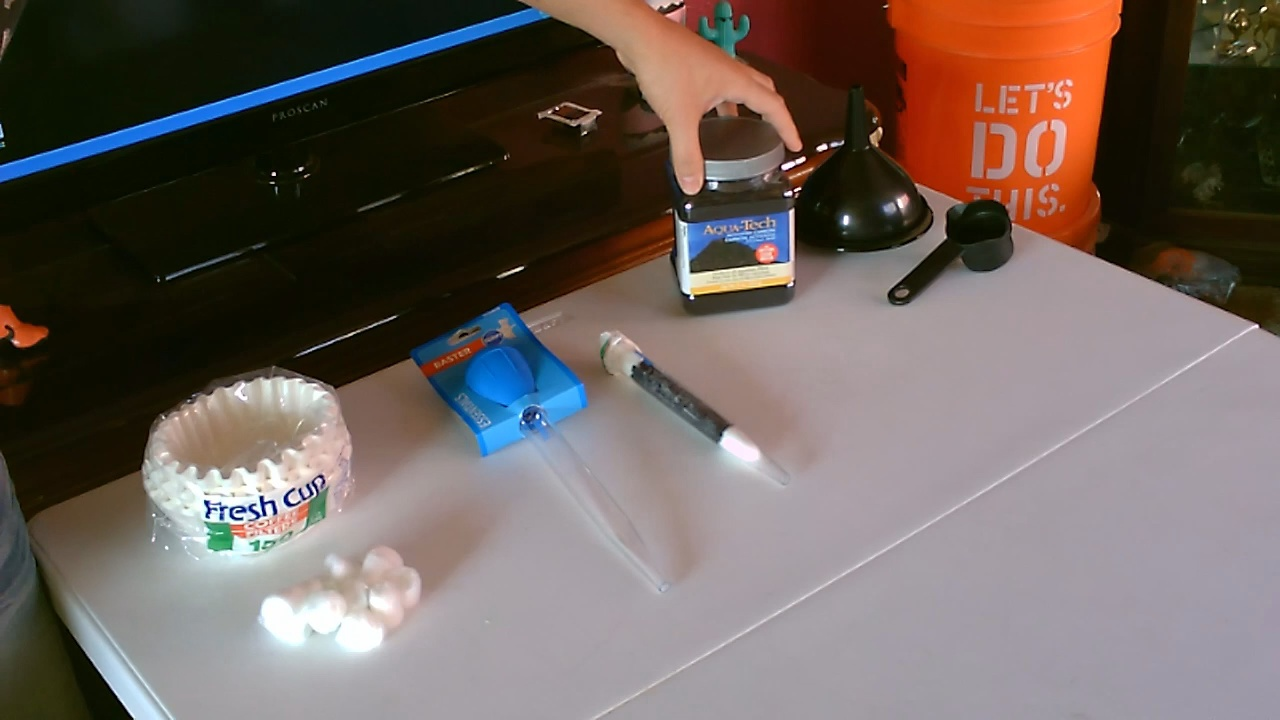
\includegraphics[width=0.6\textwidth]{DIY/materials-1.jpg}
    \caption{Step-1:- required materials}
    \label{fig:market}
\end{figure}


\begin{figure}[h!]
    \centering
    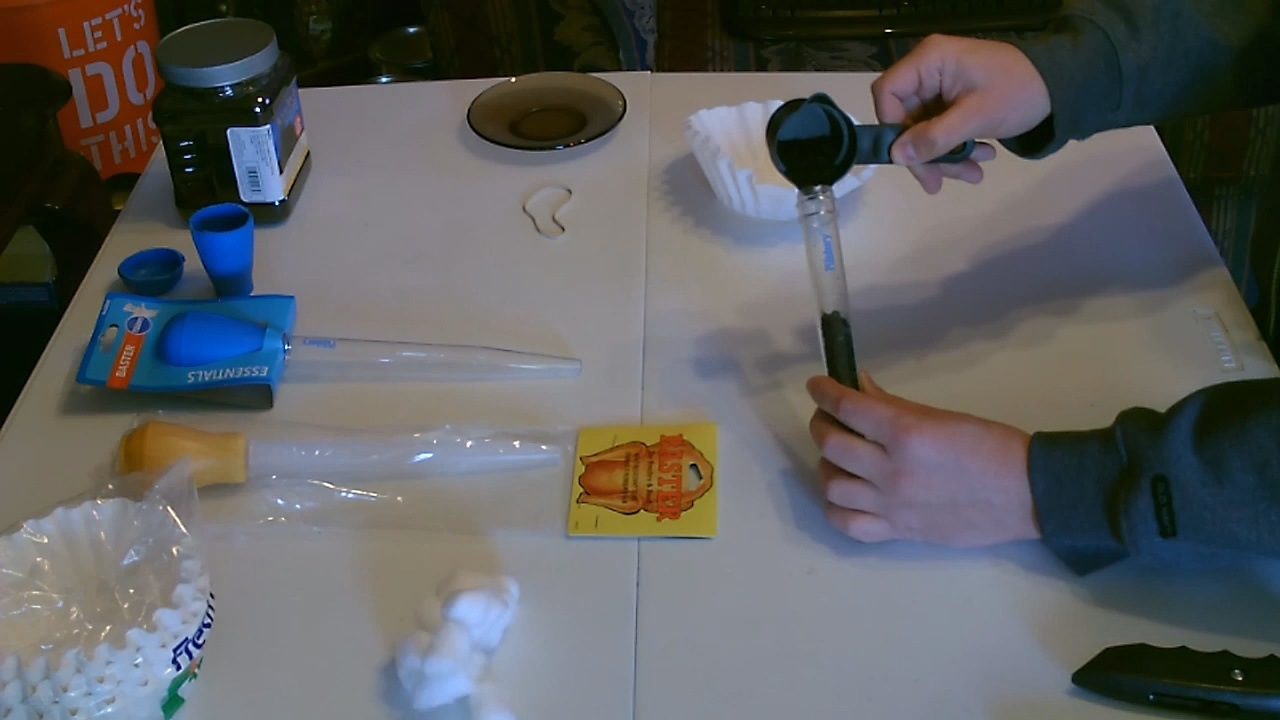
\includegraphics[width=0.6\textwidth]{DIY/materials-4.jpg}
    \caption{Step-2:-Insert a medical cotton into the tube and Add activated coal(Wash the coal before adding it into the tube) into the tube}
    \label{fig:market}
\end{figure}

\begin{figure}[h!]
    \centering
    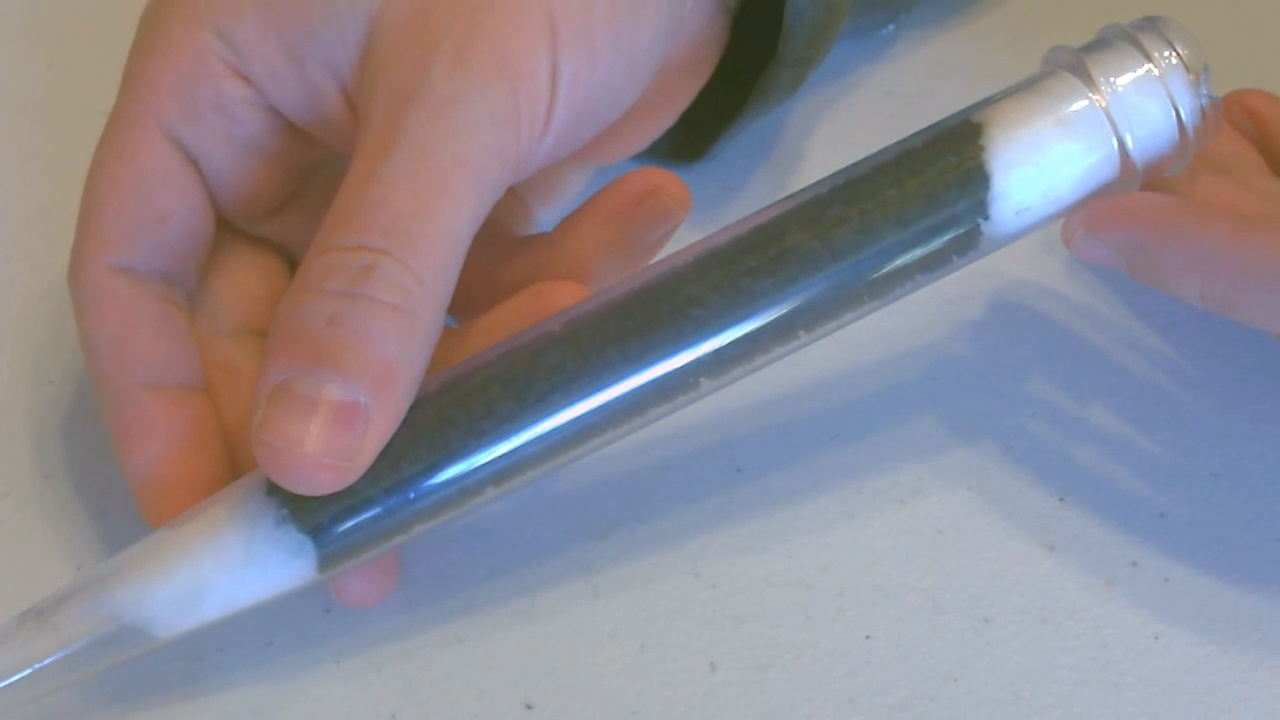
\includegraphics[width=0.6\textwidth]{DIY/materials-5jpg.jpg}
    \caption{Step-3:- insert another medical cotton into the tube}
    \label{fig:market}
\end{figure}

\begin{figure}[h!]
    \centering
    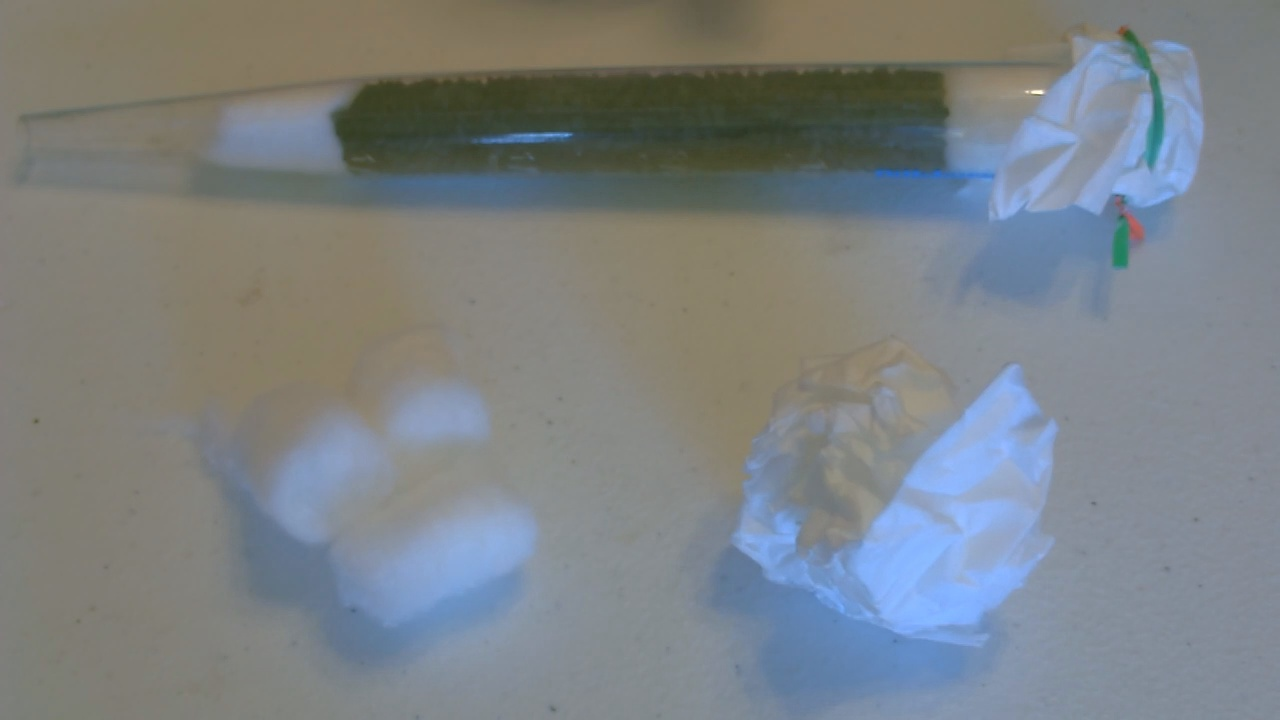
\includegraphics[width=0.6\textwidth]{DIY/material-6.jpg}
    \caption{Step-4:- add a coffee filter paper}
    \label{fig:market}
\end{figure}

\begin{figure}[h!]
    \centering
    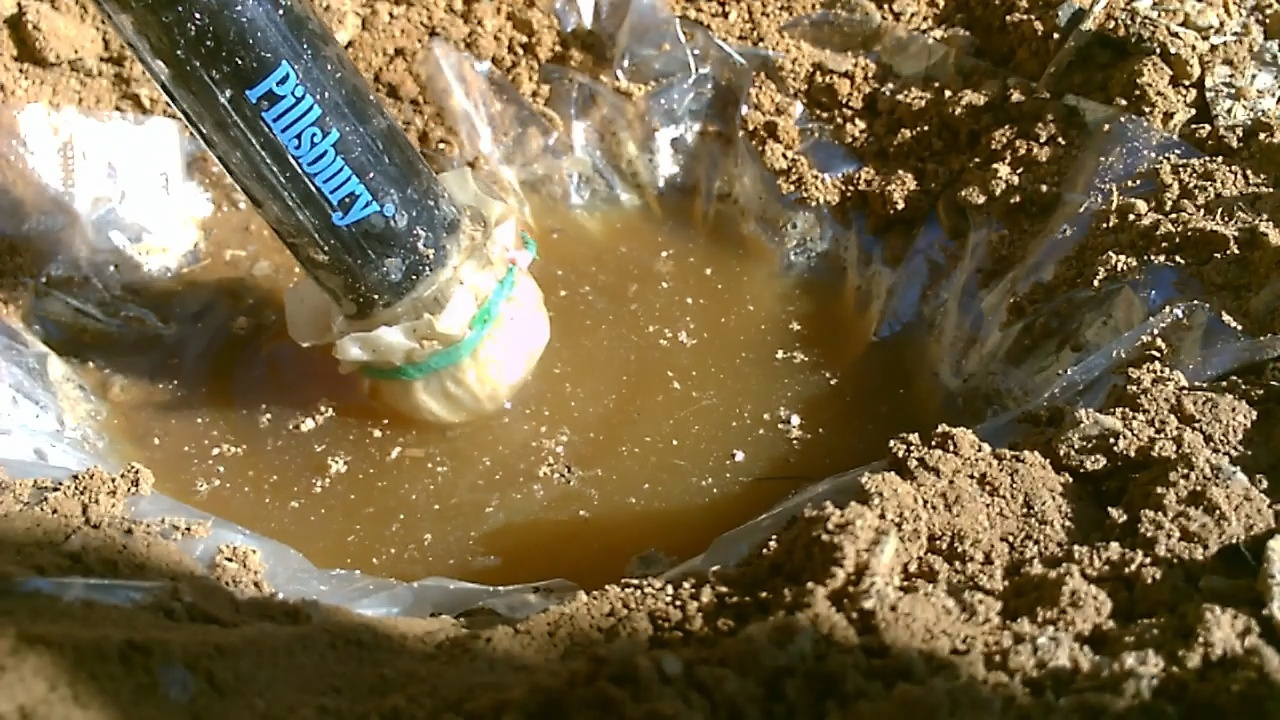
\includegraphics[width=0.6\textwidth]{DIY/material-7.jpg}
    \caption{Step-5:- for testing purposes it filters out most of the contaminants}
    \label{fig:market}
\end{figure}

\begin{figure}[h!]
    \centering
    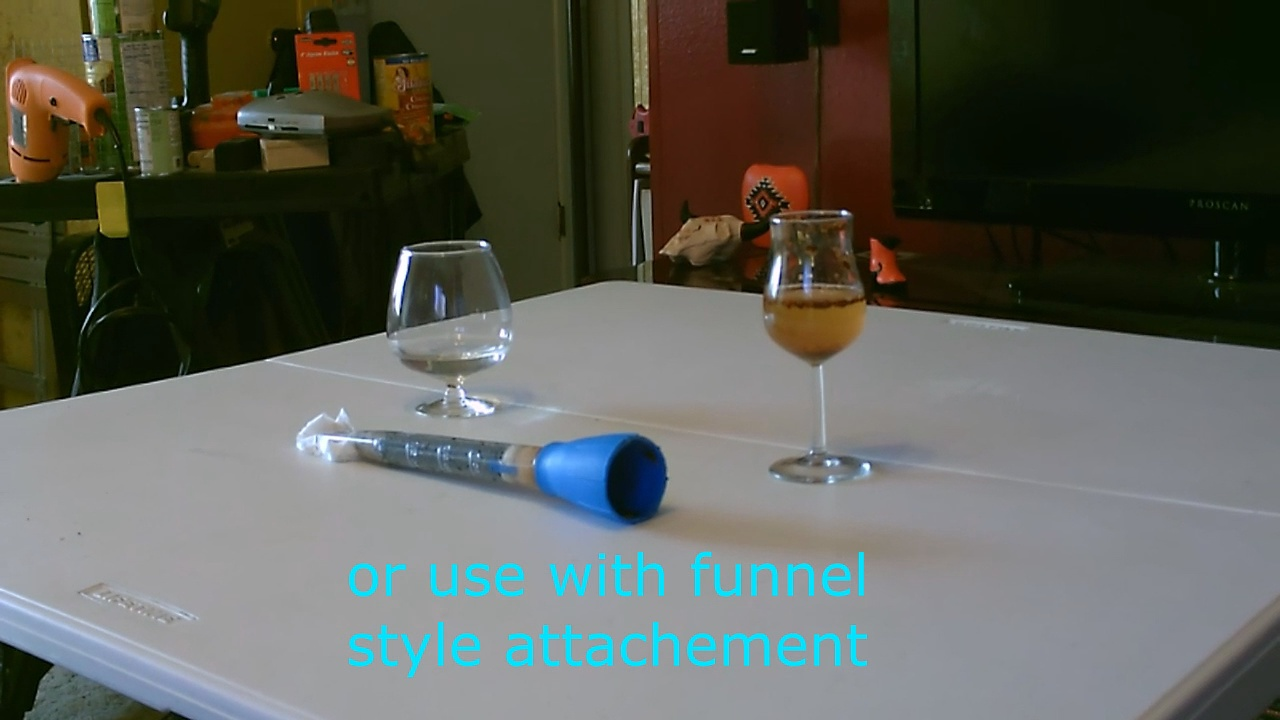
\includegraphics[width=0.6\textwidth]{DIY/material-8.jpg}
    \caption{Step-6:- you can add funnel for filtration (optional)}
    \label{fig:market}
\end{figure}


\end{document}
